\documentclass[a4paper,11pt]{article}

\usepackage[T1]{fontenc}
\usepackage[utf8]{inputenc}
\usepackage{graphicx}
\usepackage{xcolor}
\usepackage{subfigure}
\usepackage{tgtermes}
\usepackage{physics}

\usepackage[
pdftitle={Computational Physics Project}, 
pdfauthor={Heng Ni},
colorlinks=true,linkcolor=blue,urlcolor=blue,citecolor=blue,bookmarks=true,
bookmarksopenlevel=2]{hyperref}
\usepackage{amsmath,amssymb,amsthm,textcomp}
\usepackage{enumerate}
\usepackage{multicol}
\usepackage{tikz}

\usepackage{geometry}
\geometry{total={210mm,297mm},
left=25mm,right=25mm,%
bindingoffset=0mm, top=20mm,bottom=20mm}

\linespread{1.3}

\newcommand{\linia}{\rule{\linewidth}{0.5pt}}

\newtheoremstyle{mytheor}
    {1ex}{1ex}{\normalfont}{0pt}{\scshape}{.}{1ex}
    {{\thmname{#1 }}{\thmnumber{#2}}{\thmnote{ (#3)}}}

\theoremstyle{mytheor}
\newtheorem{defi}{Definition}

\makeatletter
\renewcommand{\maketitle}{
\begin{center}
\vspace{2ex}
{\huge \textsc{\@title}}
\vspace{1ex}
\\
\linia\\
\@author \hfill \@date
\vspace{4ex}
\end{center}
}
\makeatother

\usepackage{fancyhdr,lastpage}
\pagestyle{fancy}
\lhead{}
\chead{}
\rhead{}
\cfoot{}
\rfoot{\thepage}
\renewcommand{\headrulewidth}{0pt}
\renewcommand{\footrulewidth}{0pt}

\begin{document}

\title{computational physics project}

\author{Heng Ni}

\maketitle

\section{Introduction}

\ \ \ \ \ \ All materials have the effect of diamagnetism, in the external magnetic field, they will have the tend to repel the magnetic field. Generally the diamagnetism of materials is often very weak, and can only be observed in low temperature and strong magnetic field conditions, but some diamagnetic materials, for example, pyrolytic graphite, has a very strong diamagnetism that can be levitated by magnets in room temperature. The force exerted on the material by external magnetic field is 
\begin{equation}
F_z = \frac{1}{\mu_0}\chi B \frac{\partial B}{\partial z},
\end{equation}
where $F_z$ is the force in vertical direction, $\chi$ is the magnetic susceptibility. In my project, the levitation is concerned, so I only consider the force in $z$ direction, in fact, it is the perpendicular direction called $c$ axis of the disk surface we are study in this project.

Moreover, the magnetic susceptibility of pyrolytic graphite changes with temperature, even noticeable at room temperature. For highly oriented pyrolytic graphite (HOPG), the magnetic susceptibility along $c$ axis is large and very small in the $a$-$b$ plane. The force on it will be changed and may lead to motion. Therefore, we can drive a HOPG to move by changing its temperature by any methods, even by light heating, which has been realized in experiments. 

\begin{figure}[!htb]
\centering
\subfigure[]{
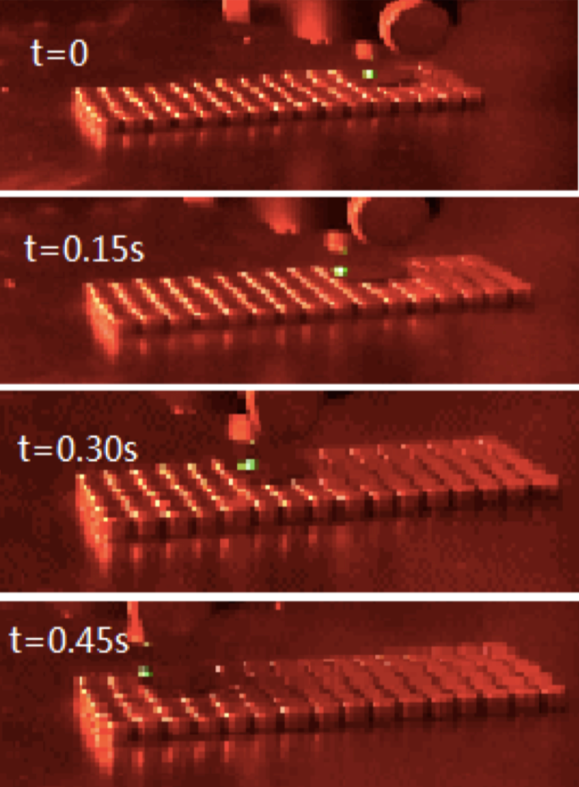
\includegraphics[width=0.3\textwidth]{figure_1a.png}}
\subfigure[]{
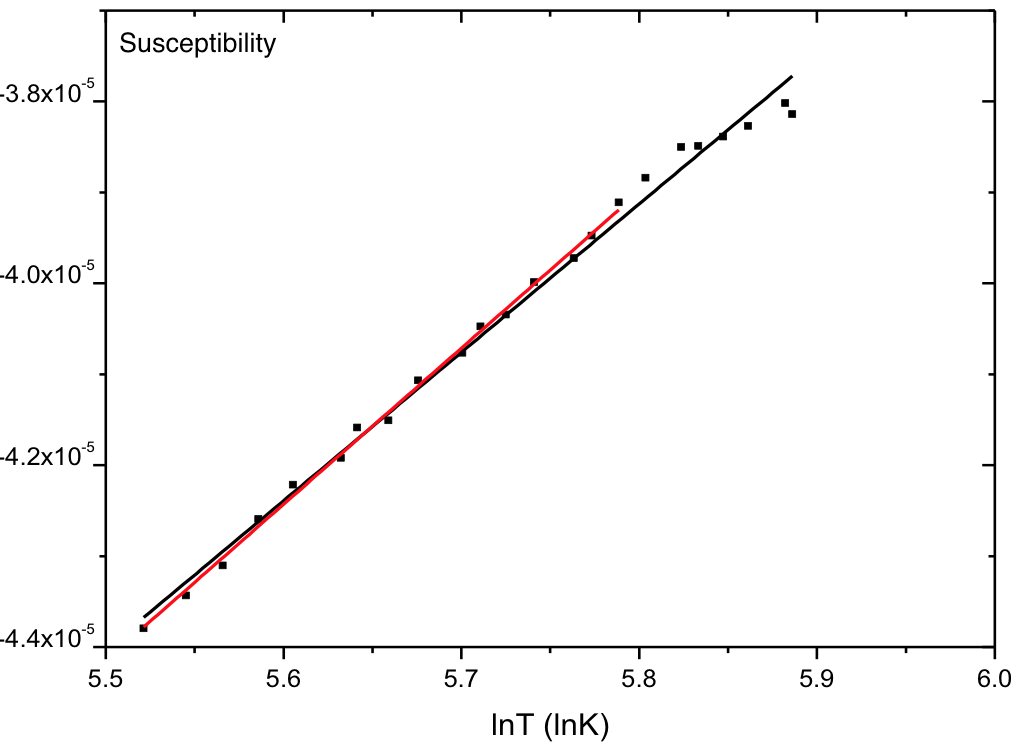
\includegraphics[width=0.5\textwidth]{figure_1b.png}}
\caption{(a) The magnetic levitated HOPG disk moving with the laser spot. (b) The result of superconducting quantum interference device (SQUID) measurement show that the susceptibility along $c$ axis have a relation of $\chi = 1.72\times10^{-5}\ln T - 1.386\times 10^{-4}$ (SI).}
\end{figure}

\clearpage

The brief explanation of this phenomenon is, when a light spot is shot on the HOPG disk, the temperature increases, which makes the absolute value of magnetic susceptibility decrease, and the levitation force decreases. This breaks the equilibrium, and the HOPG disk moves. More precisely, if we heat the disk only at one part and the temperature distribution is not uniform, the magnetic force on disk is also not uniform, which makes the disk, as a rigid body, rotate with angle $\theta$. Because the magnetic force is also perpendicular to the disk, the disk now have a horizontal component $F\cdot \sin \theta$ that drive the disk to move with the light spot, and in the same direction.

In this project, I simulated the phenomenon based on the analysis above, and separate the problem into two parts, one is to obtain the temperature distribution of the disk by solving heat equation, and the other is to turn the conditions of heat into dynamic problem and show the movement of disk. 

\section{Methods and Algorithms}
\subsection*{Heat Equation}

\ \ \ \ \ \ The disk is very thin so the $c$ axis direction can be neglected, so the heat equation can be written as
\begin{equation}
\frac{\partial u}{\partial t} = D \left( \frac{\partial^2u}{\partial x^2} + \frac{\partial^2u}{\partial y^2} \right) + q.
\end{equation}
The function of $u$ represents temperature, $D$ is the diffusivity of pyrolytic graphite, and $q$ is the source or sink function used to simulate the input light heating and output heat into the environment. 

Use the explicit method to solve the equation, so each time evolution step is
\begin{equation}
u_{j,l}^{n+1} = u_{j,l}^n + \alpha \left( \delta_x^2 u_{j,l}^n + \delta_y^2 u_{j,l}^n \right),
\end{equation}
or use Crank-Nicolson method that combines explicit and implicit to make the calculation more stable:
\begin{equation}
u_{j,l}^{n+1} = u_{j,l}^n + \frac{1}{2}\alpha \left( \delta_x^2 u_{j,l}^{n+1} + \delta_x^2 u_{j,l}^n + \delta_y^2 u_{j,l}^{n+1} + \delta_y^2 u_{j,l}^n \right),\\
\end{equation}
here,
\begin{align}
\alpha &\equiv \frac{D \Delta t}{\Delta^2},\\
\Delta &\equiv \Delta x = \Delta y,\\
\delta_x^2 u_{j,l}^n &\equiv u_{j+1,l}^n - 2u_{j,l}^n + u_{j-1,l}^n.
\end{align}
For wave equation, it is shown that explicit method is unconditionally unstable and should not be used, but for heat equation, based on von Neumann analysis, we have the conditionally stability and the condition is 
\begin{equation}
\Delta t < \frac{\Delta^2}{2D},
\end{equation}
so if this condition is satisfied, the results are still correct. The explicit method is simple and straight forward, but the Crank Nicolson method involves matrix calculation and linear equation solution, since we use the $u^{n+1}$ neighbors of next step to calculate $u^{n+1}$, the process is not simple as explicit as $\vec u^{n+1} = B\vec u^{n}$, but to solve the linear equations $A\vec u^{n+1} = B\vec u^{n}$. This is clear for one dimension, but when dealing with two or higher dimensional problem, each component of the matrices is no more number but also matrix, making the process complicated and time-consuming, therefore, we use Crank-Nicolson method only for one dimensional problem.

The source or sink function $q$ should have the dimension of temperature over time, and its physical meaning is heat flux divided by the material constants density $rho$ and specific heat capacity $c_p$, given by
\begin{equation}
\rho c_p \frac{\partial T}{\partial t} - \nabla \cdot (k \nabla T) = \dot Q,
\end{equation}
where $\dot Q$ is the heat flux. So $q$ can be defined as the input light energy times some constants. However, there is also heat loss, which I treat as heat radiation here, according to Stefan-Boltzmann Law, 
\begin{equation}
j = \sigma T^4,
\end{equation}
and here the heat loss should be
\begin{equation}
j = \sigma (T^4 - T_{s}^4),
\end{equation}
so the heat loss depends on temperature difference between the disk and the surrounding environment. The constants here have the relation:
\begin{equation}
D = \frac{k}{\rho c_p},
\end{equation}
$k$ is the thermal conductivity, so I use to $k/D$ to derive $\rho c_p$ as a more commonly used constant. 

The boundary condition should be non-flux, which means I should choose Neumann boundary condition, making the ghost zones on the boundary have the same values updated to their neighbors with each time step taken. 
\begin{equation}
u_{0}^{n} = u_{1}^{n}, u_{N}^{n} = u_{N-1}^{n}.
\end{equation}
As for the initial condition, $u$ for the whole disk can be set as zero to be uniform, and then the light heat comes in and some heats radiate away, the system evolves. 

Because the disk have round shape, the ghost zones and boundary are more complicated, to solve this, use a matrix to represent the round shape of the disk, components within have value ones, otherwise zeros. I first find the boundary along $x$ direction and save it by zeros and ones in a matrix, then along $y$ direction, add them up so I get the matrix of ghost zones marked by one or two. the components which have value two have two neighbors inside the disk. When copy the values of ghost zones, use the shape matrix to restrict their their neighbors, and then use ghost matrix take average. So I realized the boundary in cartesian coordinate.

\clearpage

\subsection*{Rigid Body Dynamics}

\ \ \ \ \ \ Once the temperature distribution of the disk is obtained, we can have the magnetic susceptibility distribution that was a constant. The nonuniform magnetic susceptibility causes a torque that will tilt the disk, and add a horizontal force on disk. 
\begin{align}
F_x &= \int \left( \frac{1}{\mu_0}\chi B \frac{\partial B}{\partial z} - \rho g \right)\mathrm{d}\vec r \cdot \sin \theta,\\
\tau &= \int \left( \frac{1}{\mu_0}\chi B \frac{\partial B}{\partial z} \right) r \mathrm{d}\vec r,
\end{align}
We choose a magnetic field along $z$ direction with a fixed gradient, because according to eqn.(1), only magnetic field with gradient can levitate the disk. With each time step, the disk repositions and rotates, since the magnetic field changes in space, so the magnetic field at each point of the disk should be recalculated and repeat the time evolution.

\begin{figure}[!htb]
\centering
\subfigure[]{
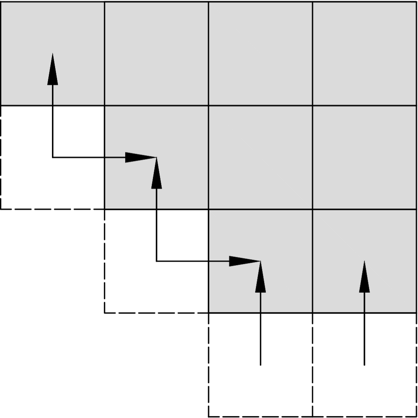
\includegraphics[width=0.4\textwidth]{figure_2a.png}}
\subfigure[]{
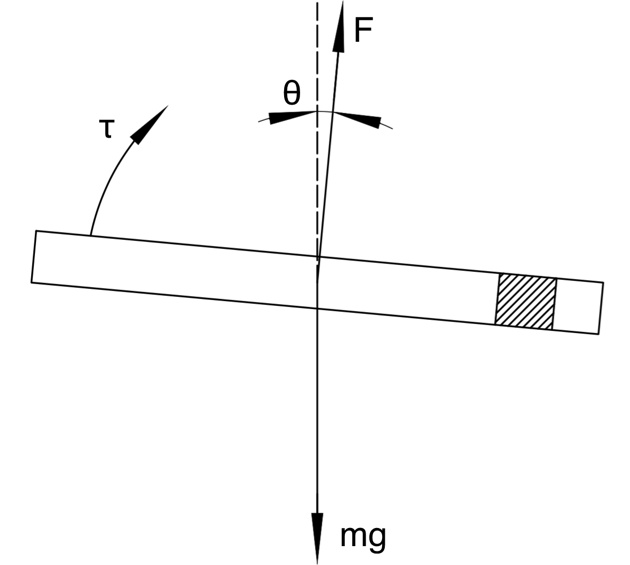
\includegraphics[width=0.45\textwidth]{figure_2b.png}}
\caption{(a) The ghost zones are no longer simply the boundary of the matrix, but these zones can be updated by finding their neighbors, there are two kinds of ghost zones, with only one neighbor or two neighbors, when updating, let them find their neighbors, sum the values and divide the number of neighbors. (b) When light spot shot on a side of HOPG disk, the equilibrium is broken, the disk tilts and the side of higher temperature lower down, giving a horizontal force.}
\end{figure}


\clearpage

\section{Results and Discussion}
\subsection*{Heat Equation}

\ \ \ \ \ \ Solving the heat equation by explicit method, I have the solution shown in Fig.3, when heating the disk, the temperature increase. The heat radiation is so weak, maybe because the temperature difference between the disk and the environment is too small, that it takes much longer time to reach the equilibrium than we consider. The explicit method have the stability condition that requires time step size to be very small, since spatial step size and diffusivity are very small, which costs lots of iterations to reach the time evolution expected.

Fig.4 shows the one dimensional HOPG temperature distribution solved by Crank-Nicolson method. I regard the HOPG as a square plate, and the light spot should be like a band, so the diffusion is only along one direction. Similarly to the two dimensional case, the temperature of HOPG is increasing and keeps a nonuniform distribution. Because the dimension and shape are different, the constants and coefficients are also different for light source.

\begin{figure}[!htb]
\centering
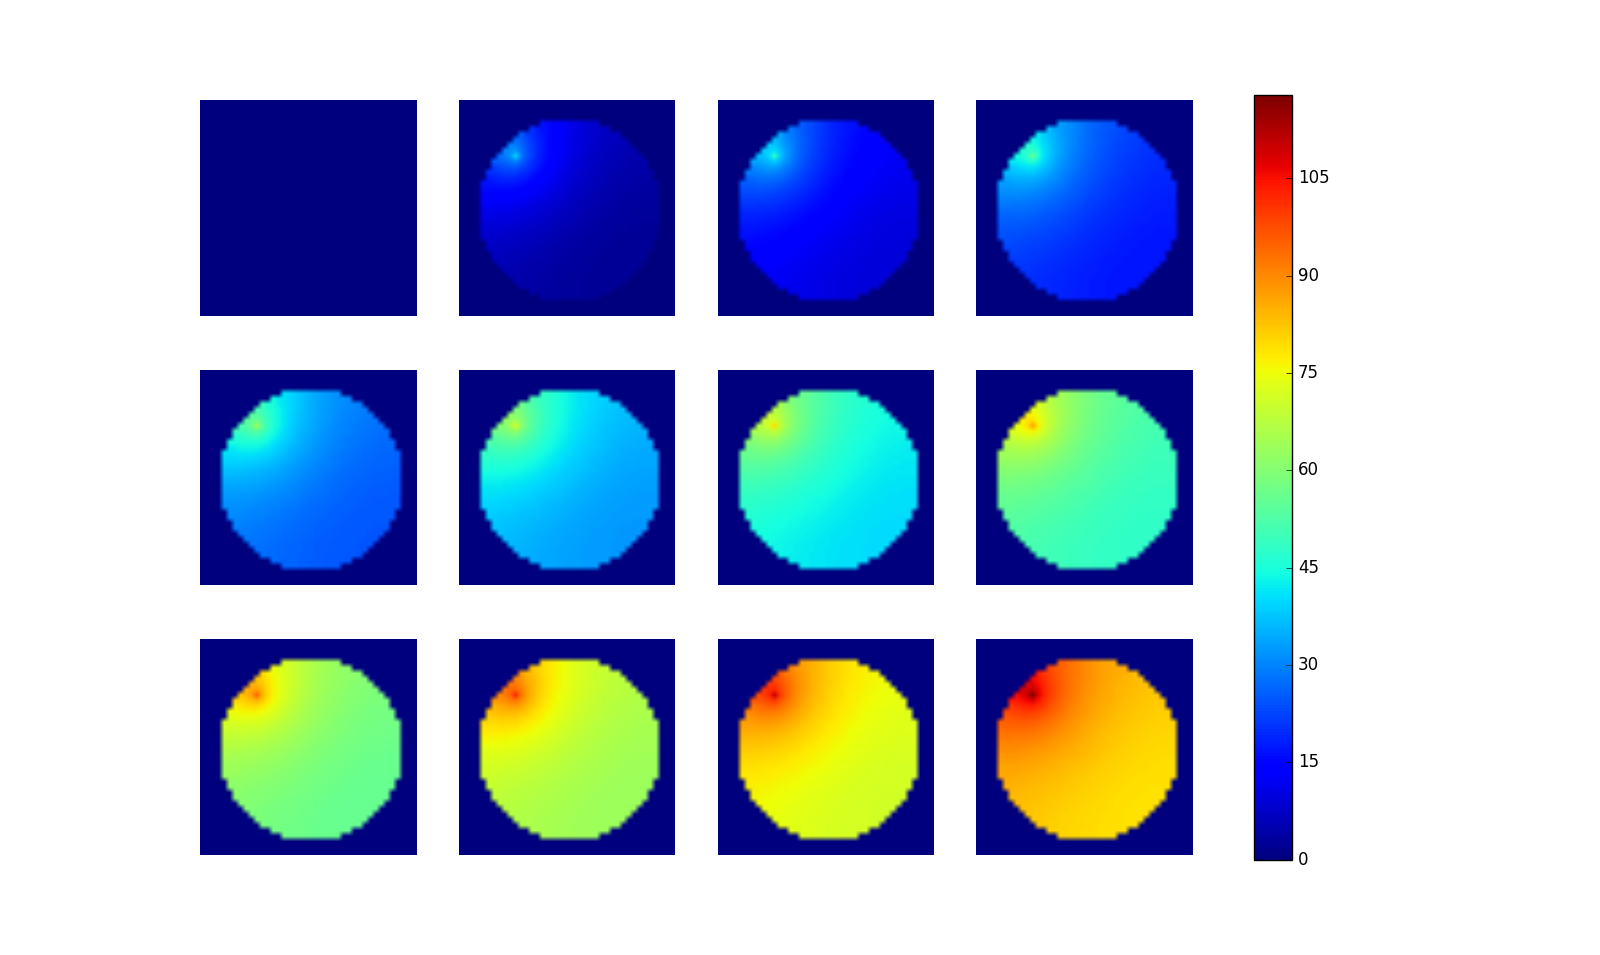
\includegraphics[width=\textwidth]{figure_3.png}
\caption{The disk is being heated at one small part and the temperature goes up as time evolves. The temperature distribution is no more uniform and keeps a difference between the heated part and the other.}
\end{figure}

\subsection*{Rigid Body Dynamics}
\ \ \ \ \ \ The motion of HOPG is shown in Fig.5, so the HOPG will follow the light spot to move horizontally, if the light spot is fixed on the same position on HOPG. The result can only be described as reasonable, but not exact, because there are arguments that are not measured precisely. For example, the energy of laser light is 340 mW, but the energy the HOPG absorbed is unknown, and the magnetic field is constructed roughly by a vertical gradient, but the experiments are carried out on a lattice of permanent magnets. Therefore, there are still much more to dig.

\clearpage

\begin{figure}[!htb]
\centering
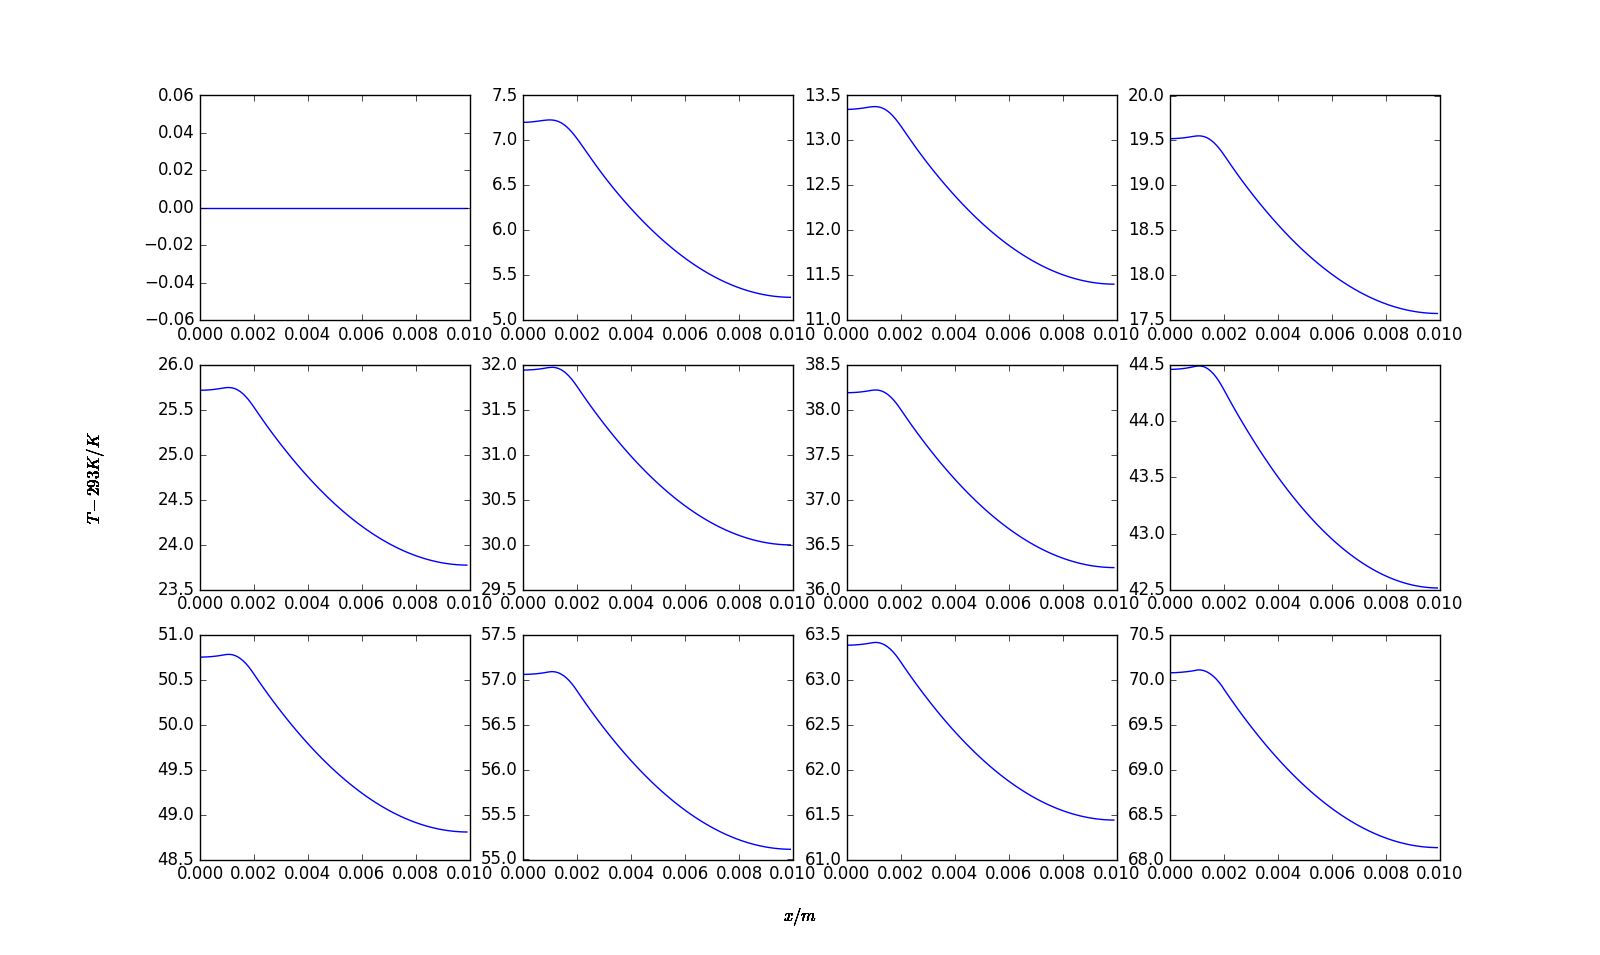
\includegraphics[width=0.9\textwidth]{figure_4.png}
\caption{The one dimensional heat equation have the similar solution of temperature distribution as the two dimensional disk.}
\end{figure}
\begin{figure}[!htb]
\centering
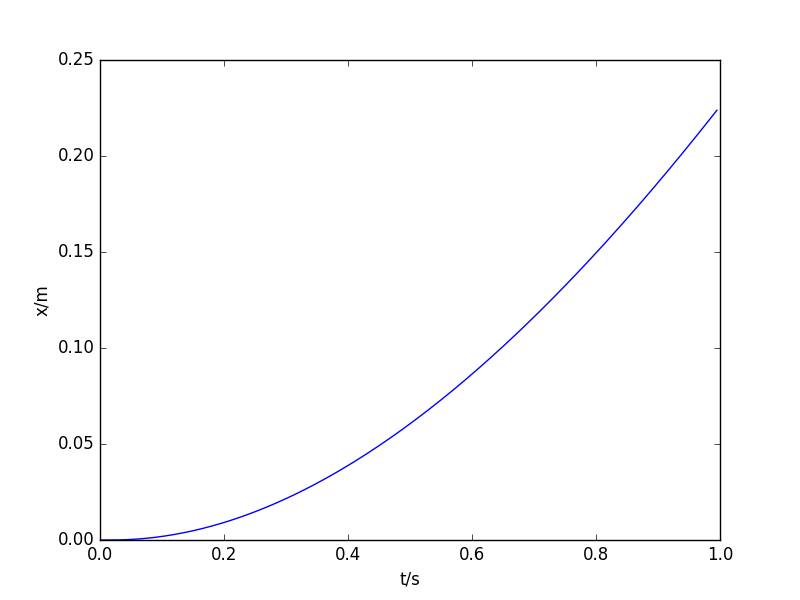
\includegraphics[width=0.9\textwidth]{figure_5.png}
\caption{The HOPG moves by the horizontal force given by magnetic field.}
\end{figure}


\end{document}